\documentclass[11pt,twocolumn]{article}

\usepackage[hmargin=1.25cm, vmargin=1.5cm]{geometry} % Document margins

\usepackage{amsmath}
\usepackage{amsthm}
\usepackage{graphicx}
\usepackage{mathtools}
\usepackage{fullpage}
\usepackage{verbatim}

\title{Brownian Dynein Model}

\newcommand{\mn}{\scalebox{0.7}[1.0]{-}}

\begin{document}

\maketitle

\section{Both bound}

\begin{figure}
  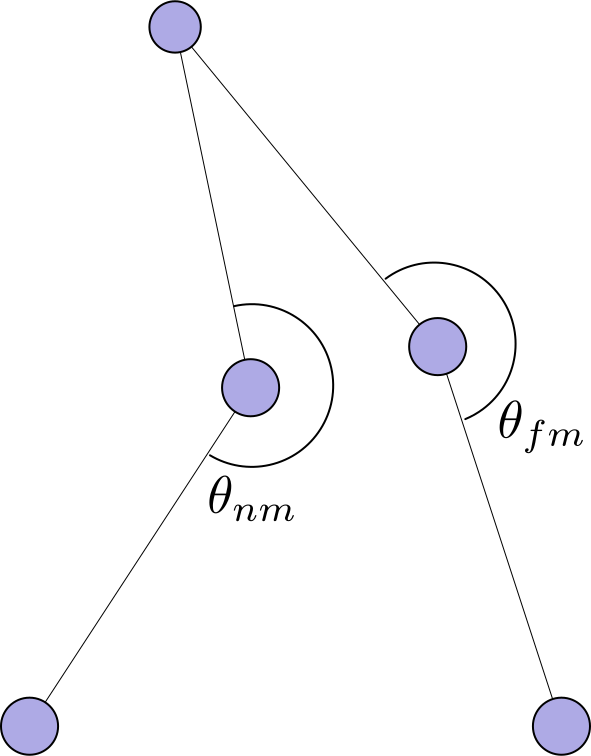
\includegraphics[width=\columnwidth]{../figures/code-bothbound}
  \caption{Angles used in both-bound case.}\label{fig:bothbound}
\end{figure}

In the both-bound case, we use two angles, as illustrated in
Fig.~\ref{fig:bothbound}.

These are the distances to the tail domain from the near and far
binding domains:
\begin{align}
  L_n &= \sqrt{L_s^2 + L_t^2 - 2L_sL_t\cos{\theta_{nm}}} \\
  L_f &= \sqrt{L_s^2 + L_t^2 - 2L_sL_t\cos{\theta_{fm}}}
\end{align}

\subsection{Nearbound and Tail coordinates}

We use two angles to determine the position of the motor domain:
\begin{align}
  \cos\theta_n &= \frac{L^2 + L_n^2 - L_f^2}{2L L_n} \\
  \sin\theta_{n} &= \sqrt{1 - \cos^2\theta_{n}} \\
  \cos\theta_{ns} &= \frac{L_s^2 + L_n^2 - L_t^2}{2L_s L_n} \\
  \sin\theta_{ns} &=
  \begin{cases}
    +\sqrt{1 - \cos^2\theta_{ns}} & \theta_{nm} < \pi \\
    -\sqrt{1 - \cos^2\theta_{ns}} & \theta_{nm} > \pi
  \end{cases}
\end{align}

and the derivatives are given by:

\begin{align}
  \frac{\partial \cos\theta_n}{\partial L_n} &= \frac{1}{L} - \frac{L^2 + L_n^2 - L_f^2}{2L L_n^2}\\
  \frac{\partial \cos\theta_n}{\partial L_f} &= -\frac{L_f}{LL_n}\\
  \frac{\partial \sin\theta_n}{\partial L_n} &= \frac{-\cos\theta_n}{\sqrt{1-\cos^2\theta_n}}
  \left(\frac{1}{L} - \frac{L^2 + L_n^2 - L_f^2}{2L L_n^2}\right)\\
  \frac{\partial \sin\theta_n}{\partial L_f} &= \frac{-\cos\theta_n}{\sqrt{1-\cos^2\theta_n}}
  \left(\frac{-L_f}{LLn}\right)\\
  \frac{\partial \cos\theta_{ns}}{\partial L_n} &= \frac{1}{L_s}
  - \frac{L_s^2 + L_n^2 - L_t^2}{2L_sL_n^2}\\
  \frac{\partial \cos\theta_{ns}}{\partial L_f} &= 0\\
  \frac{\partial \sin\theta_{ns}}{\partial L_n} &=
  \begin{cases}
    \frac{-\cos\theta_{ns}}{\sqrt{1-\cos^2\theta_{ns}}}
    \left(\frac{1}{L_s} - \frac{L_s^2+L_n^2-L_t^2}{2LL_n^2}\right) & \theta_{nm} < \pi \\
    \frac{\cos\theta_{ns}}{\sqrt{1-\cos^2\theta_{ns}}}
    \left(\frac{1}{L_s} - \frac{L_s^2+L_n^2-L_t^2}{2LL_n^2}\right) & \theta_{nm} > \pi
  \end{cases}\\
  \frac{\partial \sin\theta_{ns}}{\partial L_f} &= 0
\end{align}

Given these definitions, the position of the motor domain is given
simply by $\cos$ and $\sin$ of $\theta_n$ and $\theta_{ns}$:
\begin{align}
  X_{nm} &= L_s\left(
  \cos\theta_n\cos\theta_{ns} - \sin\theta_n\sin\theta_{ns}
  \right)
  \\
  Y_{nm} &= L_s\left(
  \cos\theta_n\sin\theta_{ns} + \sin\theta_n\cos\theta_{ns}
  \right)
  \\
  X_{t} &= L_n\cos\theta_n\\
  Y_{t} &= L_n\sin\theta_n\\
\end{align}

Looking at their derivatives gives:

\begin{multline}
  \frac{dX_{nm}}{dL_n} = L_s\Big(
  \cos\theta_n\frac{d\cos\theta_{ns}}{dL_n}
  + \cos\theta_{ns}\frac{d\cos\theta_{n}}{dL_n} \\
  - \sin\theta_n\frac{d\sin\theta_{ns}}{dL_n}
  - \sin\theta_{ns}\frac{d\sin\theta_{n}}{dL_n}
  \Big)\\
\end{multline}

\begin{multline}
  \frac{dY_{nm}}{dL_n} = L_s\Big(
  \cos\theta_n\frac{d\sin\theta_{ns}}{dL_n}
  + \sin\theta_{ns}\frac{d\cos\theta_{n}}{dL_n} \\
  + \sin\theta_n\frac{d\cos\theta_{ns}}{dL_n}
  + \cos\theta_{ns}\frac{d\sin\theta_{n}}{dL_n}
  \Big)
\end{multline}

\begin{multline}
  \frac{dX_{nm}}{dL_f} = L_s\Big(
  \cos\theta_n\frac{d\cos\theta_{ns}}{dL_f}
  + \cos\theta_{ns}\frac{d\cos\theta_{n}}{dL_f} \\
  - \sin\theta_n\frac{d\sin\theta_{ns}}{dL_f}
  - \sin\theta_{ns}\frac{d\sin\theta_{n}}{dL_f}
  \Big)
\end{multline}

\begin{multline}
  \frac{dY_{nm}}{dL_f} = L_s\Big(
  \cos\theta_n\frac{d\sin\theta_{ns}}{dL_f}
  + \sin\theta_{ns}\frac{d\cos\theta_{n}}{dL_f} \\
  + \sin\theta_n\frac{d\cos\theta_{ns}}{dL_f}
  + \cos\theta_{ns}\frac{d\sin\theta_{n}}{dL_f}
  \Big)
\end{multline}

\begin{align}
  \frac{dX_{t}}{dL_n} &= \cos\theta_n\\
  \frac{dY_{t}}{dL_n} &= \sin\theta_n\\
  \frac{dX_{t}}{dL_f} &= 0\\
  \frac{dY_{t}}{dL_f} &= 0\\
\end{align}

The corresponding C++ code could look like:
\begin{verbatim}
  dXnm_dLn = Ls*(cosAn*dcosAns_dLn
                 + cosAns*dcosAn_dLn
                 - sinAn*dsinAns_dLn
                 - sinAns*dsinAn_dLn);
\end{verbatim}
Basically, we have lots of chain rules.\\

We then create a system of equations by equating velocities from Brownian dynamics to the velocities
we derived above:

\onecolumn

\begin{align}
  \dot{X}_{nm} &= \frac{1}{\gamma} \Big(F_{xml} + \mn \lambda_{ns}(X_{bm} - X_{bb})
  + \lambda_{nt}(X_{t } - X_{bm}) \Big) + R_{xml}
  &=& \frac{X_{nm}}{Ln}\dot{L}_n + \frac{X_{nm}}{Lf}\dot{L}_f\\
  \dot{X}_{t } &= \frac{1}{\gamma} \Big(F_{xt } + \mn \lambda_{nt}(X_{t } - X_{bm})
  + \lambda_{ft}(X_{fm} - X_{t }) \Big) + R_{xt }
  &=& \frac{X_{t}}{Ln}\dot{L}_n + \frac{X_{t}}{Lf}\dot{L}_f\\
  \dot{X}_{fm} &= \frac{1}{\gamma} \Big(F_{xmr} + \mn \lambda_{ft}(X_{fm} - X_{t })
  + \lambda_{fs}(X_{fb} - X_{fm}) \Big) + R_{xmr}
  &=& \frac{X_{fm}}{Ln}\dot{L}_n + \frac{X_{fm}}{Lf}\dot{L}_f
\end{align}

\begin{align}
  \dot{Y}_{nm} &= \hspace{1cm} \frac{1}{\gamma} \Big(F_{yml} + \mn \lambda_{ns}(Y_{bm} - Y_{bb})
  + \lambda_{nt}(Y_{t } - Y_{bm}) \Big) + R_{yml}
  &= \frac{Y_{nm}}{Ln}\dot{L}_n + \frac{Y_{nm}}{Lf}\dot{L}_f\\
  \dot{Y}_{t}  &= \hspace{1cm} \frac{1}{\gamma} \Big(F_{yt } + \mn \lambda_{nt}(Y_{t } - Y_{bm})
  + \lambda_{ft}(Y_{fm} - Y_{t }) \Big) + R_{yt }
  &= \frac{Y_{t}}{Ln}\dot{L}_n + \frac{Y_{t}}{Lf}\dot{L}_f\\
  \dot{Y}_{fm} &= \hspace{1cm} \frac{1}{\gamma} \Big(F_{ymr} + \mn \lambda_{ft}(Y_{fm} - Y_{t })
  + \lambda_{fs}(Y_{fb} - Y_{fm}) \Big) + R_{ymr}
  &= \frac{Y_{fm}}{Ln}\dot{L}_n + \frac{Y_{fm}}{Lf}\dot{L}_f
\end{align}

\twocolumn

\begin{figure}
  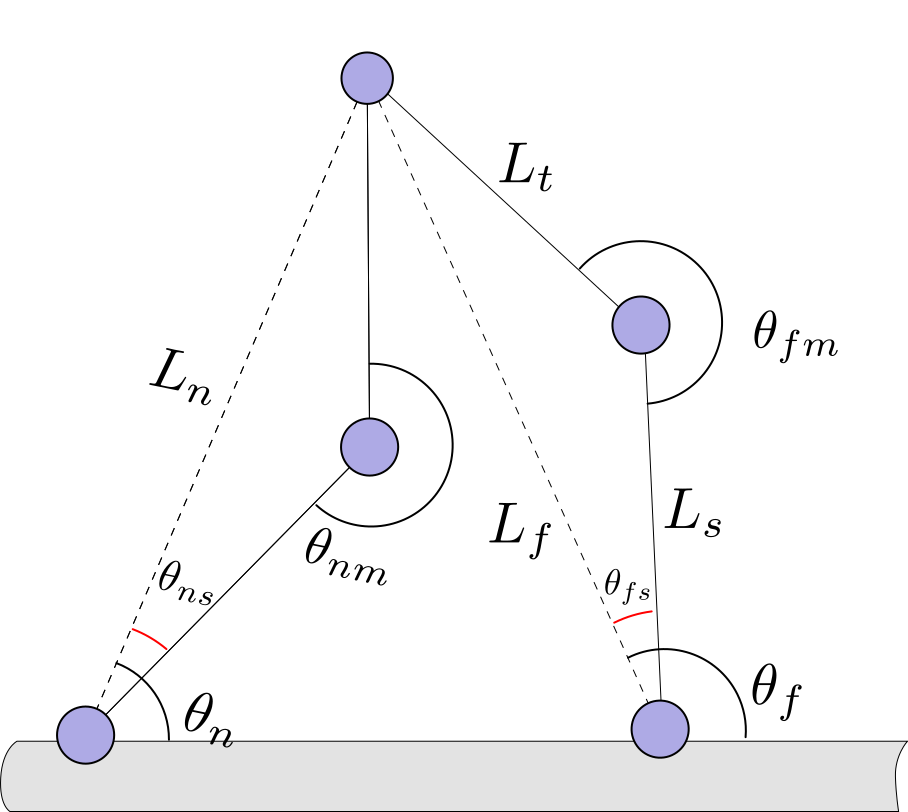
\includegraphics[width=\columnwidth]{../figures/similar-bothbound}
  \caption{Angles used in both-bound case.}\label{fig:similar}
\end{figure}

\subsection{Farbound coordinates}
The farbound coordinates are defined similarly (but not quite) to the nearbound coordinates, with
$L_n$ and $L_f$ coordinates switched places.
\begin{align}
  \cos\theta_f &= -\frac{L^2 + L_f^2 - L_n^2}{2L L_f}\\
  &\Bigg( \mbox{Or equivalently...   }
  \cos\left(\pi - \theta_f\right) &= \frac{L^2 + L_f^2 - L_n^2}{2L L_f}\Bigg)\\
  \sin\theta_{f} &= \sqrt{1 - \cos^2\theta_{f}} \\
  \cos\theta_{fs} &= \frac{L_s^2 + L_f^2 - L_t^2}{2L_s L_f} \\
  \sin\theta_{fs} &=
  \begin{cases}
    +\sqrt{1 - \cos^2\theta_{fs}} & \theta_{fm} < \pi \\
    -\sqrt{1 - \cos^2\theta_{fs}} & \theta_{fm} > \pi
  \end{cases}
\end{align}

\onecolumn

\section{Matrix Solution via Mathematica}
Here we convert the above system into matrix form, solve it in Mathematica and list the results.

\[
\begin{pmatrix}
  -\frac{X_{nm}}{Ln} & -\frac{X_{nm}}{Lf}
  & -\frac{X_{nm}-X_{nb}}{\gamma} & \frac{X_{t}-X_{nm}}{\gamma} & 0 & 0\\
  -\frac{X_{t}}{Ln} & -\frac{X_{t}}{Lf}
  & 0 & -\frac{X_{t}-X_{nm}}{\gamma} & \frac{X_{fm}-X_{t}}{\gamma} & 0\\
  -\frac{X_{fm}}{Ln} & -\frac{X_{fm}}{Lf}
  & 0 & 0 & -\frac{X_{fm}-X_{t}}{\gamma} & \frac{X_{fb}-X_{fm}}{\gamma}\\
  -\frac{Y_{nm}}{Ln} & -\frac{Y_{nm}}{Lf}
  & -\frac{Y_{nm}-Y_{nb}}{\gamma} & \frac{Y_{t}-Y_{nm}}{\gamma} & 0 & 0\\
  -\frac{Y_{t}}{Ln} & -\frac{Y_{t}}{Lf}
  & 0 & -\frac{Y_{t}-Y_{nm}}{\gamma} & \frac{Y_{fm}-Y_{t}}{\gamma} & 0\\
  -\frac{Y_{fm}}{Ln} & -\frac{Y_{fm}}{Lf}
  & 0 & 0 & -\frac{Y_{fm}-Y_{t}}{\gamma} & \frac{Y_{fb}-Y_{fm}}{\gamma}\\
\end{pmatrix}
\begin{pmatrix}
  \dot{L}_n\\
  \dot{L}_f\\
  \lambda_{ns}\\
  \lambda_{nt}\\
  \lambda_{ft}\\
  \lambda_{fs}\\
\end{pmatrix}
=
\begin{pmatrix}
  -\frac{F_{xml}}{\gamma} - R_{xml}\\
  -\frac{F_{xt}}{\gamma} - R_{xt}\\
  -\frac{F_{xmr}}{\gamma} - R_{xmr}\\
  -\frac{F_{yml}}{\gamma} - R_{yml}\\
  -\frac{F_{yt}}{\gamma} - R_{yt}\\
  -\frac{F_{ymr}}{\gamma} - R_{ymr}\\
\end{pmatrix}
\]

\twocolumn

\section{One bound}

\begin{figure}
  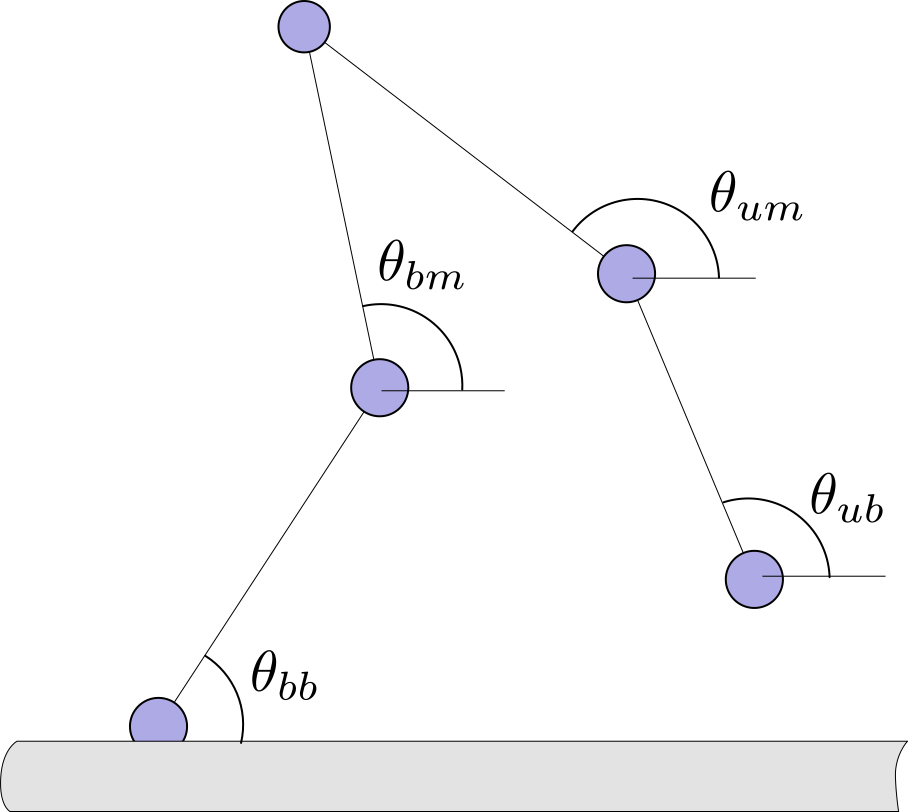
\includegraphics[width=\columnwidth]{../figures/code-onebound}
  \caption{Angles used in one-bound case.}\label{fig:onebound}
\end{figure}

In the one-bound case, we use four angles, as illustrated in
Fig.~\ref{fig:onebound}.

\end{document}
